\documentclass[letterpaper]{article}
\usepackage[submission]{aaai2027}
\usepackage[hyphens]{url}
\usepackage{graphicx}
\urlstyle{rm}
\def\UrlFont{\rm}
\usepackage{natbib}
\usepackage{caption}
\frenchspacing
\usepackage{algorithm}
\usepackage{algorithmic}
\usepackage{booktabs}
\usepackage{amsmath}
\usepackage{amssymb}
\usepackage{multirow}
\usepackage{float}
\usepackage{placeins}


\pdfinfo{
/TemplateVersion (2027.1)
}

\setcounter{secnumdepth}{0}

\title{Beyond Semantic IDs: Finite-Beam Output Support in Generative Recommendation}
\author{Anonymous Submission}
\affiliations{}

\begin{document}

\maketitle

\begin{abstract}
Generative recommendation (GR) retrieves items by autoregressively decoding discrete Semantic IDs (SIDs) over learned codebooks, typically with finite-width beam search. We study how this practical search budget distributes retrieval support across items. We distinguish three quantities that are often conflated: whether an item has a unique code, whether it can be scored by an interface, and whether it actually appears in a finite top-$K$ output. To isolate the output interface, we introduce two continuous-query methods in a shared frozen item space: CQG-Single generates one query in a single forward pass, while CQG-AR autoregressively generates continuous residuals that refine the query. Both remove the item-token vocabulary and retrieve by dense scoring or approximate nearest-neighbor search. Controlled diagnostics reveal a checkpoint- and budget-specific finite-beam reachability ceiling and, in some popularity strata and evaluated checkpoints, a depth-dependent pattern in which SID decoding can be competitive at shallow $K$ while continuous retrieval becomes more favorable deeper in the ranked list. Under a unified seven-seed ML-1M protocol with valid-prefix constrained decoding, CQG-Single achieves R@10 \(0.3104\), compared with \(0.2996\) for TIGER, and is higher in all seven indexed runs (exact sign-flip \(p=.0156\)). CQG-AR provides an architecture-matched test of whether autoregression requires discrete SID outputs. Our results motivate returned-list-size-matched evaluation of discrete and continuous retrieval interfaces rather than treating catalog-wide scoreability as empirical top-$K$ coverage.
\end{abstract}

\section{Introduction}

\begin{figure*}[t]
\centering
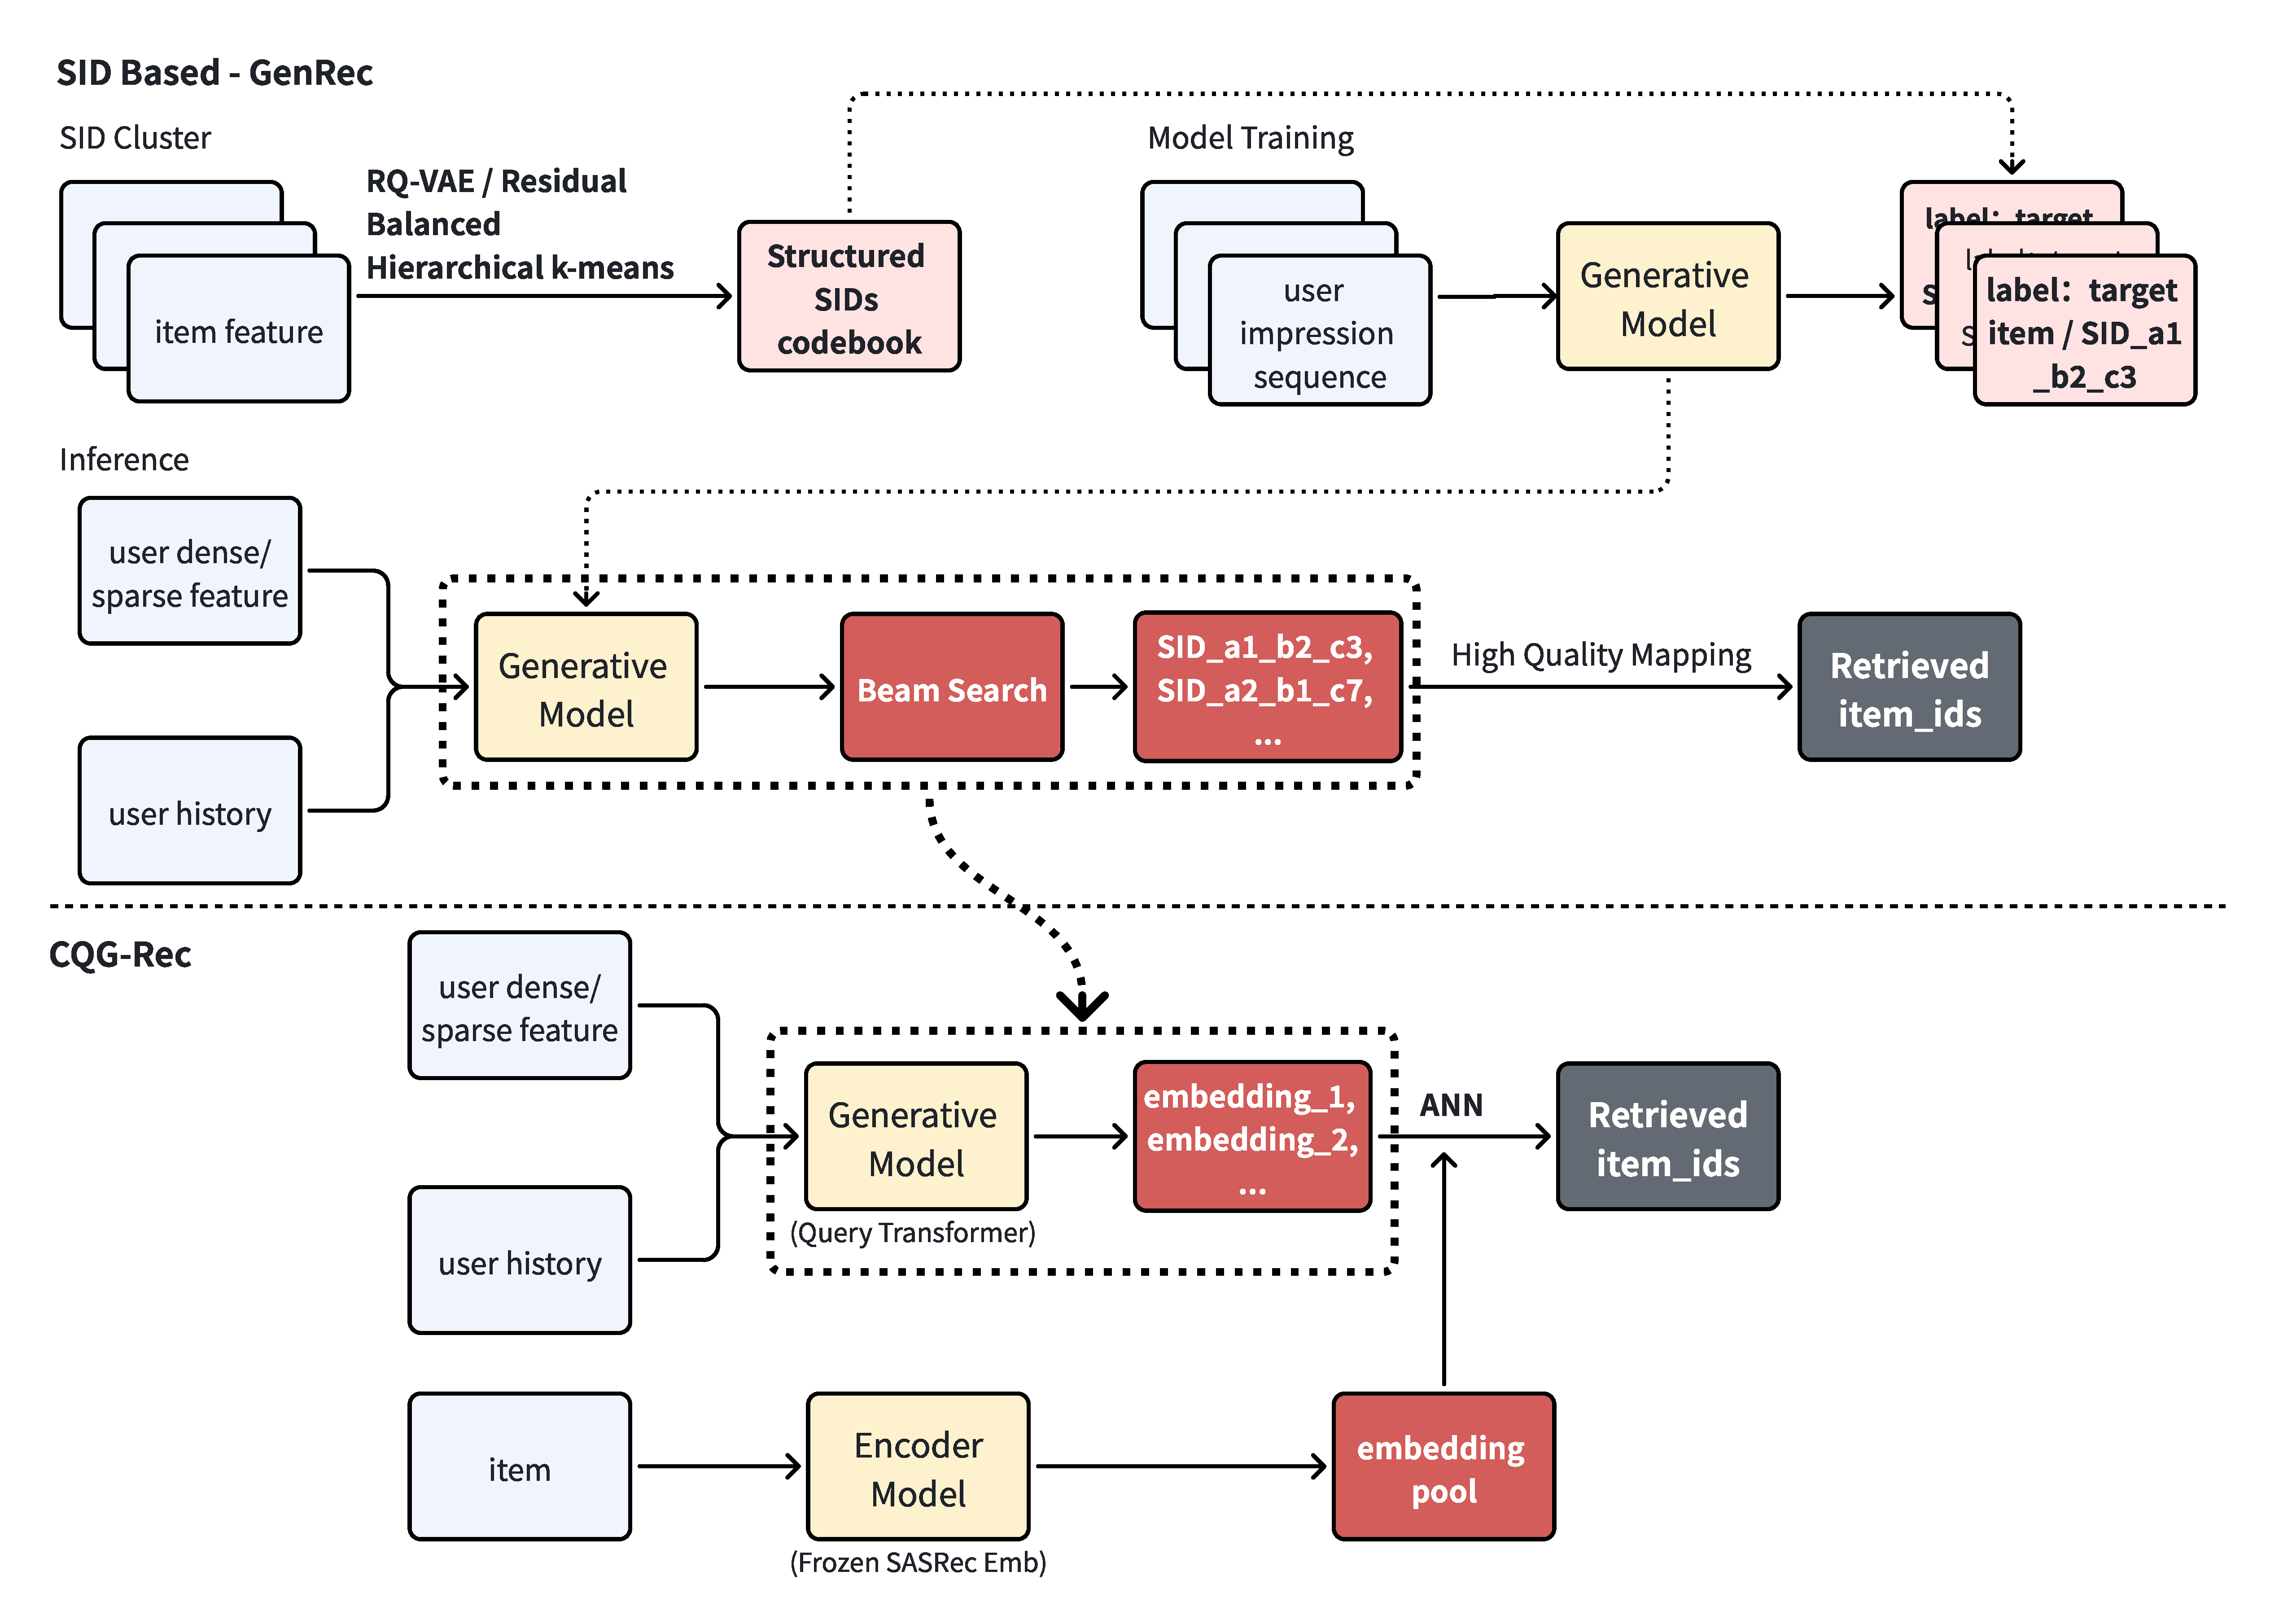
\includegraphics[width=0.75\textwidth]{Figures/fig1_1_pipeline.pdf}
\caption{Inference interfaces for SID retrieval, CQG-Single, and CQG-AR. 
SID retrieval autoregressively generates discrete code tokens and explores
catalog-valid paths with finite-width, valid-prefix beam search. CQG-Single produces one
continuous query in a single forward pass, whereas CQG-AR autoregressively 
generates residual updates that refine a continuous query. Both CQG variants 
retrieve from the same frozen item embedding index by dense scoring or ANN, 
without an item-token vocabulary or code-to-item lookup.}
\label{fig:pipeline}
\end{figure*}

Generative recommendation (GR) retrieves items by generating symbolic identifiers rather than directly scoring the entire catalog. The most influential instance of this paradigm is Semantic-ID (SID) recommendation: items are first quantized into discrete code sequences, and an autoregressive model decodes those sequences conditioned on user attributes and interaction history \citep{rajput2023tiger,zheng2024letter,wang2024eager}. This formulation converts recommendation into a sequence-generation problem, and supports constrained decoding through a trie, ensuring that the generated token sequence corresponds to a valid item.

This marks a substantial architectural shift from conventional sequential recommenders. Models such as SASRec encode user histories, user features, and item representations, then score candidate items discriminatively \citep{kang2018sasrec}. In SID-based generative recommendation, the output interface is instead moved into a language-model-style generator: a decoder is trained to emit the SID sequence. Larger pretrained language models can provide useful generic knowledge and may benefit from scaling behavior as model and data size increase \citep{kaplan2020scaling}, but SID-based GR still requires three additional system components: First, items must be compressed into a finite hierarchical identifier space, using vector-quantization methods such as VQ-VAE \citep{vandenoord2017vqvae}, residual quantization as in RQ-VAE \citep{lee2022rqvae}, residual or balanced hierarchical clustering, or industrial generative retrieval designs such as OneRec \citep{deng2025onerec}. Second, the generator must be trained either by adapting a pretrained LLM through continued pretraining and supervised fine-tuning, where SID tokens become a new vocabulary that must be aligned with the LLM's semantic space, or by training a smaller decoder-only model from scratch, which sacrifices pretrained knowledge for a cleaner SID prediction objective. Third, inference decodes SID sequences from user features and sequential history, then maps the generated codes to item IDs or expands them through item-to-item retrieval. (Figure~\ref{fig:pipeline})

These steps introduce two practical bottlenecks. The first is coverage and updateability: a catalog item is useful only if its SID can be generated and mapped back to the item, but newly created items may cause semantic drift between the clustering model labeling and the item meaning. The second is support imbalance: a finite hierarchical SID space is a compromise for representing an open-ended catalog. Items are not distributed uniformly across SID leaves, semantic partitions can overlap, and the generated SID set may fail to recall enough valid items even when the related item catalog itself is large.

Because SID inference explores only a prefix-limited subset of the code tree,
we define a \emph{checkpoint- and budget-specific finite-beam reachability
ceiling} as the target-support upper bound induced by a fixed trained model and finite beam budget, even when
the held-out item has a valid code.

This support limitation motivates a checkpoint- and popularity-dependent
\emph{crossover pattern}. At shallow retrieval depth, SID models can perform
well because autoregressive decoding concentrates probability mass on
high-confidence paths. On rare ML-1M targets for the evaluated seed-42
checkpoints, TIGER outperforms a continuous alternative at R@10; at some
deeper $K$, the continuous model catches up or overtakes. We treat this as an
operating-point-dependent empirical pattern, not as proof that a per-user hit
rate equals an item-level catalog-coverage ceiling.

To isolate this mechanism, we study two complementary continuous-query
formulations. \textbf{CQG-Single} is a deliberately minimal vocabulary-free
model that maps user context to one continuous query in a frozen item space.
\textbf{CQG-AR} retains a TIGER-like autoregressive decoder but replaces
SID-token prediction with continuous residual generation, feeding each
generated residual back to refine the query. Both retrieve by dense scoring
or approximate nearest-neighbor (ANN) search without a code-to-item lookup.
CQG-Single tests the simplest continuous interface, while CQG-AR controls for
autoregressive model structure.

Our contributions are:
\begin{itemize}
    \item \textbf{Finite-search diagnostics.} For a fixed checkpoint and search
    budget, we distinguish unique-code assignment, target-conditioned beam
    support, catalog-wide scoreability, and empirical union-of-top-$K$
    coverage, and stratify the output-based quantities by item popularity.
    \item \textbf{Conditional crossover pattern.} In some popularity strata
    and evaluated checkpoints, SID decoding can achieve higher shallow
    Recall@$K$, while continuous retrieval can overtake at deeper $K$ under a
    matched returned-list size.
    \item \textbf{Parallel continuous-query methods.} We introduce CQG-Single, a one-step continuous retriever, and CQG-AR, an autoregressive continuous decoder. Their comparison separates the effect of autoregression from the effect of a discrete SID vocabulary.
    \item \textbf{Controlled empirical study.} Across ML-1M, Amazon Beauty, and Amazon Sports, we analyze retrieval quality, reranked performance, loss functions, LLM backbone failures, and tokenization instability while limiting scalability claims to the tested catalog sizes.
\end{itemize}

\section{Related Work}

\textbf{Semantic-ID generative recommendation.}
TIGER \citep{rajput2023tiger} introduced hierarchical Semantic IDs using
residual vector quantization and autoregressive decoding. Later work improves
identifier learning and alignment through collaborative semantics, textual
IDs, differentiable indexing, or soft identifiers
\citep{zheng2024letter,wang2024eager,tan2024idgenrec,fu2026diger,li2026unigrec}.
These methods differ in code construction but retain a structured output
interface that typically uses constrained autoregressive decoding. We study
how finite-width search allocates support over that interface, rather than
proposing another discrete tokenizer. This distinction also separates
successful code assignment from successful code retrieval at inference time.

\textbf{Finite search support and popularity.}
Autoregressive tree generation can impose correlation constraints on
representable item distributions \citep{hou2026expressiveness}, while
training-side studies note that tail tokens receive fewer updates. We examine
the complementary inference-side question: even with a valid, nearly unique
code, does a target enter a finite beam? We measure target-conditioned beam
support, returned-list-size-matched catalog coverage, and popularity-stratified behavior,
carefully separating these quantities. In particular, a high unique-code rate
does not imply that every target enters a user's beam, and a target-conditioned
hit rate does not equal catalog coverage. Our experiments treat these as
distinct diagnostics of a trained model and its search budget.

\textbf{Vocabulary-free and continuous recommendation.}
DiffuRec, DreamRec, and ContRec use diffusion or continuous latent generation
\citep{10.1145/3631116,yang2023dreamrec,qu2026contrec}, while GPT4Rec generates
textual retrieval queries \citep{li2023gpt4recgenerativeframeworkpersonalized}. CQG-Single provides a minimal
continuous-query control, and CQG-AR adds step-wise residual refinement. Their
purpose is to separate autoregression from discrete SID output, not to claim
dense retrieval itself as novel. This paired design asks whether step-wise
generation requires discrete identifier tokens: CQG-Single removes both the
token vocabulary and serial decoding, whereas CQG-AR preserves serial
generation but replaces tokens with continuous residual updates.

\textbf{Sequential, dense, and hybrid retrieval.}
GRU4Rec, SASRec, and BERT4Rec score catalog items from interaction histories
\citep{hidasi2016gru4rec,kang2018sasrec,sun2019bert4rec}; dual encoders are
established in retrieval and recommendation
\citep{huang2013dssm,covington2016youtube}. Generative retrieval instead
decodes identifiers \citep{tay2022dsi,wang2022nci}, and LIGER combines dense
and generative retrieval \citep{yang2024liger}. These lines establish both
catalog scoring and identifier decoding as known retrieval interfaces.
Our contribution is therefore a controlled comparison in a shared frozen item
space, using CQG-Single and CQG-AR to distinguish finite SID output support
from autoregressive modeling without attributing the comparison to a larger
item encoder or an additional reranker.
\section{Method}

\subsection{Problem Formulation}

Let $\mathcal{I}$ be a catalog of $N$ items and let user $u$ have a chronological interaction sequence $s_u=(i_1,\ldots,i_t)$. The task is to retrieve the next item $i_{t+1}$. SID-based GR maps each item $i$ to a discrete code sequence $z_i=(z_{i,1},\ldots,z_{i,L})$ and trains an autoregressive model $p(z_i\mid s_u)$. Inference uses beam search over valid code prefixes.

Both of our continuous methods assume a frozen item embedding matrix $E\in\mathbb{R}^{N\times d}$, where each row $e_i$ is an L2-normalized item vector. They condition on the same user context $c_u$ available to the SID decoder, including the sequential item history and, when available, demographic features. They differ in whether the continuous output is produced in one step or autoregressively.

\subsection{CQG-Single: Single-Step Continuous Query Generation}

CQG-Single learns a single-step query generator $f_\theta$:
\begin{equation}
q_u = f_\theta(c_u), \quad q_u\in\mathbb{R}^d .
\end{equation}
The recommendation score is cosine similarity:
\begin{equation}
\operatorname{score}(u,i)=q_u^\top e_i .
\end{equation}
The top-K items are retrieved by exact dense scoring or ANN search. Every item in $E$ is scoreable by construction, although catalog-wide scoreability does not guarantee that every item will empirically appear in a finite top-$K$ list.

The query generator is a causal Transformer that maps the final valid history
state back into the shared item space. Unlike SID decoding, it produces the
retrieval query in one forward pass without an item-token vocabulary.

\subsection{CQG-AR: Autoregressive Continuous Query Generation}

CQG-AR retains an autoregressive decoder but replaces discrete SID-vocabulary prediction with continuous residual generation. At decoding step $\ell$, the decoder conditions on the user context and all previous continuous outputs:
\begin{align}
h_\ell &= D_\phi(c_u,\Delta_{<\ell}),\\
\Delta_\ell &= W_{\mathrm{AR}}h_\ell,\\
\hat e_u^{(\ell)} &=
\operatorname{norm}\!\left(\hat e_u^{(\ell-1)}+\Delta_\ell\right).
\end{align}
We initialize the cumulative query as
\(\hat e_u^{(0)}=\mathbf{0}\).
The generated residual $\Delta_\ell$ is projected back into the decoder input space and appended as the next autoregressive input. After $L$ steps, the refined query $\hat e_u^{(L)}$ retrieves items from the same frozen embedding matrix $E$. Thus CQG-AR preserves the conditional, step-wise decoding structure of SID retrieval while removing the SID vocabulary, codebook lookup, and discrete beam expansion.
% We use $L=3$ as an architecture-matched control for the three-level SID output, rather than assuming that three continuous refinements are intrinsically necessary. The $L=1$ setting is its single-step boundary and provides a controlled link to CQG-Single.

\subsection{Training Objectives}

We evaluate four CQG objectives: full-catalog CE, sampled CE, in-batch
InfoNCE, and MSE. For CQG-Single, $q_b$ below is the single generated query;
for CQG-AR, it is the final refinement $\hat e_b^{(L)}$. In the primary
CQG-AR configuration, only the final query receives direct CE supervision;
intermediate supervision is used only in the decoding-depth ablation.

\textbf{Full-catalog cross-entropy.}
Our primary objective treats retrieval as classification over all items:
\begin{equation}
\mathcal{L}_{\mathrm{CE}}
= -\frac{1}{B}\sum_{b=1}^{B}
\log
\frac{\exp(q_b^\top e_b^+/\tau)}
{\sum_{j=1}^{N}\exp(q_b^\top e_j/\tau)} ,
\end{equation}
where $\tau=0.07$. CE gives complete catalog visibility at training time but costs $O(N)$ per step.

\textbf{Sampled cross-entropy.}
To control training-time catalog visibility, sampled CE replaces the full
denominator with the positive item and a sampled set
\(\mathcal S_b\) of negatives:
\begin{equation}
\mathcal{L}_{\mathrm{sCE}}
=-\frac{1}{B}\sum_{b=1}^{B}\log
\frac{\exp(q_b^\top e_b^+/\tau)}
{\exp(q_b^\top e_b^+/\tau)+
\sum_{j\in\mathcal S_b}\exp(q_b^\top e_j/\tau)} .
\end{equation}
The reported control uses 256 sampled negatives.

\textbf{In-batch InfoNCE.}
InfoNCE treats the other target items in the minibatch as negatives:
\begin{equation}
\mathcal{L}_{\mathrm{NCE}}
=-\frac{1}{B}\sum_{b=1}^{B}\log
\frac{\exp(q_b^\top e_b^+/\tau)}
{\sum_{j\in\mathcal B}\exp(q_b^\top e_j^+/\tau)} .
\end{equation}

\textbf{Mean-squared error.}
We also test direct embedding regression:
\begin{equation}
\mathcal{L}_{\mathrm{MSE}}
=\frac{1}{B}\sum_{b=1}^{B}\|q_b-e_b^+\|_2^2 .
\end{equation}
MSE preserves geometric alignment but yields lower retrieval accuracy than CE
in our experiments. BPR is used to pretrain the shared SASRec item encoder,
not as one of the reported CQG objectives.

\subsection{Retrieval, Reranking, and Contrast with SID}

Standalone CQG-Single ranks items according to $q_u^\top e_i$, while CQG-AR uses $(\hat e_u^{(L)})^\top e_i$. Exact catalog scoring can be replaced by ANN search, such as FAISS, for large catalogs. Our CQG-AR experiments retrieve only with the final query \(\hat e_u^{(L)}\); merging candidates from intermediate or interest-specific queries is an untested extension. In our retrieve-and-rerank evaluation, the continuous generator retrieves 100 candidates, which are then reranked by a pretrained SASRec model. In contrast, SID retrieval requires codebook learning, autoregressive discrete decoding, beam search, and code-to-item lookup; a finite beam explores only a restricted subset of valid code paths (Figure~\ref{fig:pipeline}). CQG-Single instead generates one continuous query, while CQG-AR preserves step-wise autoregressive generation with continuous outputs. Both directly query the item embedding index without introducing an item-token vocabulary.

% \subsection{Contrast with SID Retrieval}

% Figure~\ref{fig:pipeline} compares the inference mechanisms. SID retrieval requires codebook learning, autoregressive discrete decoding, beam search, and code-to-item lookup. Under a finite beam budget, only a restricted subset of valid code paths is explored. CQG-Single uses single-step continuous generation, whereas CQG-AR retains autoregressive decoding with continuous outputs. Both continuous variants query a dense index without introducing an item-token vocabulary.

\section{Experiments}

\subsection{Experimental Setup}

\textbf{Datasets.}
We use MovieLens-1M (ML-1M), Amazon Beauty, and Amazon Sports. ML-1M is the primary controlled diagnostic because its catalog is small enough for exact full-catalog scoring. Beauty and Sports test cross-domain behavior. Our processed Sports split (21,519 users and 10,693 non-padding items) differs from the commonly reported 5-core split used by TIGER, LETTER, and EAGER; consequently, we do not directly compare our Sports values with their published numbers. We exclude Yelp because its SID and continuous baselines are not aligned under one evaluation protocol.

\begin{table}[t]
\centering
\small
\begin{tabular}{lrrrr}
\toprule
Dataset & Users & Items & Interactions & Density \\
\midrule
ML-1M & 6,040 & 3,416 & 999K & 4.84\% \\
Beauty & 22,363 & 12,101 & 198K & 0.07\% \\
Sports & 21,519 & 10,693 & \(\sim\)178K & 0.08\% \\
\bottomrule
\end{tabular}
\caption{Dataset statistics. Item counts exclude the padding row. Density is
defined as $|\mathcal{R}|/(|\mathcal{U}||\mathcal{I}|)$, where
$\mathcal{R}$ is the set of observed interactions, $\mathcal{U}$ the users,
and $\mathcal{I}$ the non-padding items. The processed Sports split differs
from the standard 5-core split used in several published SID studies, so its
results are treated as within-paper diagnostics.}
\label{tab:data}
\end{table}

\begin{figure}[t]
\centering
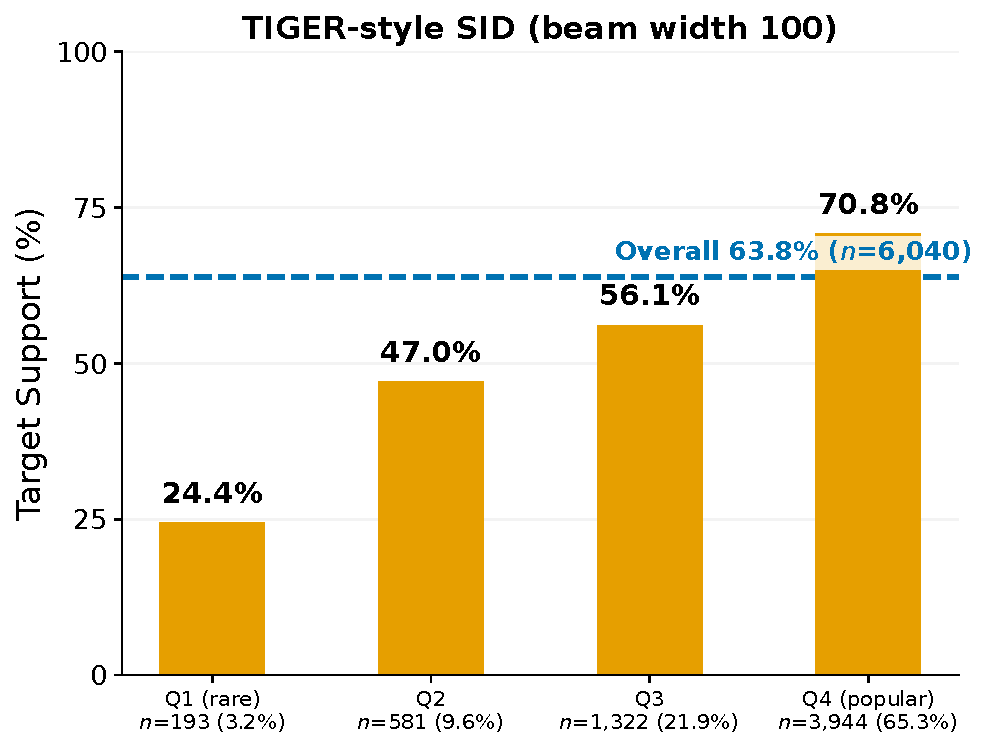
\includegraphics[width=0.9\columnwidth]{Figures/fig3_reachability.pdf}
\caption{ML-1M TargetInOutput@100 by target-popularity quartile (seed 42).
All methods return 100 valid, distinct, history-filtered items; TIGER uses
valid-prefix constrained decoding. Bars are user weighted, whereas
Table~\ref{tab:target-support-comparison} reports item-balanced quartile values.}
\label{fig:reachability}
\end{figure}

\textbf{Protocol.}
We use leave-one-out evaluation: the last item is held out for testing, the second-to-last item for validation, and earlier interactions for training. Historical items are excluded from ranking. We report Recall@K and NDCG@K, primarily for $K\in\{10,30,50,70,90\}$ in reachability analysis and $K\in\{5,10,20\}$ in cross-dataset evaluation.
\begin{figure*}[t]
\centering
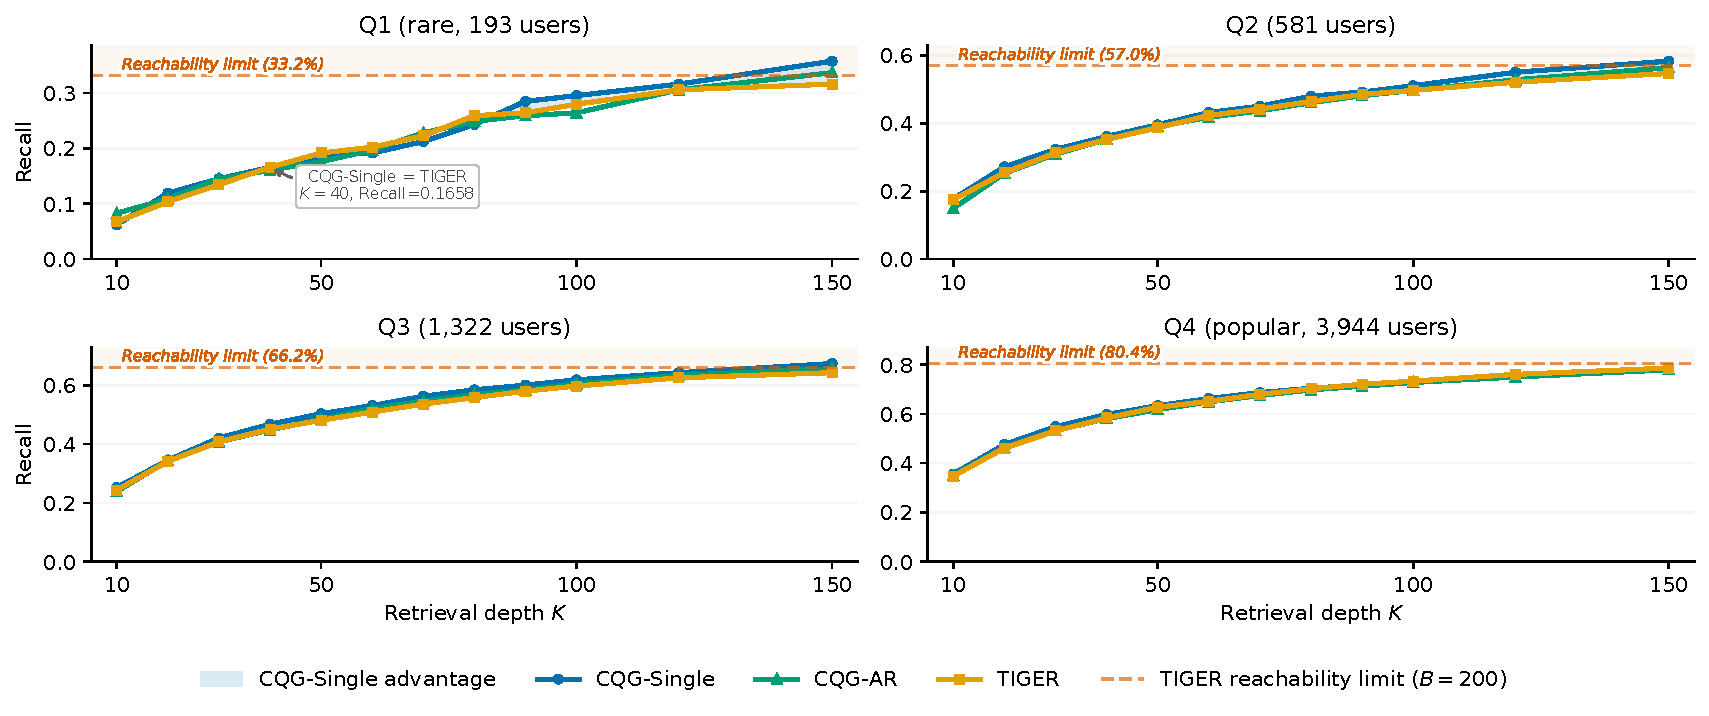
\includegraphics[width=\textwidth]{Figures/fig2_crossover.pdf}
\caption{Measured per-quartile Recall@$K$ curves on ML-1M, seed 42.
CQG-Single and CQG-AR are shown separately; light-blue shading highlights
intervals in which CQG-Single exceeds TIGER. Vermillion dashed lines show
TIGER's user-weighted TargetSupport@200 within each quartile, which upper-bounds
Recall@$K$ for any ranking restricted to the same decoded beam; the light
vermillion regions above them are unreachable for the evaluated model--beam
pair. The Q1 annotation marks the exact measured
CQG-Single--TIGER tie at $K=40$ (Recall $=0.1658$). Every
curve point uses saved per-user output at
$K\in\{10,20,\ldots,100,120,150\}$; no metric point is interpolated. All
three methods return exactly 200 valid, distinct, history-filtered items per user.}
\label{fig:crossover}
\end{figure*}
\medskip
\noindent\textbf{Baselines}\par
\smallskip
We compare against SASRec \citep{kang2018sasrec}, TIGER-style SID retrieval, and reported SID results from TIGER, LETTER, and EAGER where protocols allow contextual comparison. We also include non-learned dense retrieval baselines: random retrieval, last-item kNN, and mean-of-5 kNN.

\textbf{Model training protocol.}
We first train a two-layer SASRec with BPR on chronological next-item pairs and select its checkpoint by full-catalog validation NDCG@10. Its 64-dimensional item embedding table is then frozen and shared by both continuous methods as the history-input table, target embedding or classifier matrix, and retrieval index. The main experiments use no textual or language-model item encoder.

\textbf{CQG-Single} is a four-layer, four-head causal Transformer with width
256. It directly generates one normalized query; the final configuration uses
full-catalog CE, with MSE and in-batch InfoNCE evaluated as ablations.
\textbf{CQG-AR} uses a four-layer, six-head causal Transformer with width 384
to autoregressively generate three residual query updates. Each residual is
fed into the next decoding step, while the cumulative query is updated by
adding the residual and then normalizing the result. In the final
configuration, only the final query receives direct full-catalog CE
supervision. The multimodal Sports diagnostic instead uses a frozen fusion of
collaborative and ImageNet-pretrained ResNet-18 features. Full implementation
details are provided in Appendix D.

\section{Results}

\subsection{Budget-Specific Finite-Beam Reachability}

For a fixed model and returned-list size $B$, target support is the fraction of test
users whose held-out target occurs anywhere in the returned list. On ML-1M,
the seed-42 TargetInOutput@100 values are 66.7\% for TIGER, 67.3\% for
CQG-Single, and 66.4\% for CQG-AR. This is a per-user quantity closely related
to Recall@100; it is not the fraction of catalog items retrieved.
Figure~\ref{fig:reachability} reports the matched popularity breakdown and
user counts.

For this fixed model--search pair, TargetSupport@$B$ is a realized ceiling on
the Recall of any downstream reranker restricted to the decoded beam: a target
that never enters the candidate set cannot be recovered later. This is a
finite-beam reachability ceiling, not an architecture-invariant claim; increasing
$B$ can raise it. CQG avoids this particular beam-exclusion mechanism because
every encoded item remains scoreable, although its finite Top-$K$ Recall is
still determined by query quality.

Table~\ref{tab:target-support-comparison} provides the returned-list-size-matched finite-output comparison. TargetInOutput@100 is user weighted. Q1--Q4 first compute the hit rate of each distinct test-target item and then average items equally within training-frequency quartiles. TargetItemSupport@200 is the fraction of distinct held-out target items retrieved for at least one associated test instance. Under the corrected constrained protocol, CQG-Single retains a small advantage in overall user-weighted TargetInOutput@100 and in all four item-balanced quartiles, whereas TIGER slightly exceeds CQG-AR overall and on rare targets. Differences in distinct-target support are also small. Union-of-output catalog coverage is reported separately in Table~\ref{tab:matched-coverage}.
Figure~\ref{fig:reachability} is user weighted, whereas the Q1--Q4 columns in
Table~\ref{tab:target-support-comparison} average distinct target items equally
within the same quartile mapping.

\begin{table*}[!t]
\centering
\small
\setlength{\tabcolsep}{4pt}
\renewcommand{\arraystretch}{0.87}
\begin{tabular}{lrrrrrr}
\toprule
& \shortstack{User-weighted\\TargetInOutput@100} &
\multicolumn{4}{c}{Item-balanced TargetInOutput@100} &
\shortstack{TargetItemSupport\\@200} \\
\cmidrule(lr){3-6}
Method & Overall & Q1 rare & Q2 & Q3 & Q4 popular & Distinct targets \\
\midrule
TIGER & 66.7\% & 25.8\% & 45.2\% & 54.0\% & 68.6\% & 78.1\% \\
CQG-Single & \textbf{67.3\%} & \textbf{26.4\%} & \textbf{46.9\%} & \textbf{56.3\%} & \textbf{70.0\%} & \textbf{78.9\%} \\
CQG-AR & 66.4\% & 24.4\% & 45.4\% & 54.8\% & 69.6\% & 78.8\% \\
\bottomrule
\end{tabular}
\caption{ML-1M finite-output support (seed 42). Overall is user weighted;
Q1--Q4 average distinct target items within training-frequency quartiles, and
the final column is the fraction of distinct targets retrieved at least once
by Top-200. Returned-list sizes and filtering are matched across methods.}
\label{tab:target-support-comparison}
\end{table*}

This result separates code assignment from target support: 99.4\% unique codes do not imply that every held-out target enters a finite returned list. Under the corrected Top-100 protocol, 33.3\% of held-out user targets do not enter the corresponding candidate list; this is not a statement that 33.3\% of catalog items are never retrieved. The distinct union-of-output catalog-coverage diagnostic is reported in Table~\ref{tab:matched-coverage}.

\subsection{Popularity-Dependent Crossover}

Table~\ref{tab:primary-comparison} provides the primary cross-dataset
comparison, while Figure~\ref{fig:crossover} examines retrieval depth and
target popularity on ML-1M; exact values and paired-bootstrap intervals are
reported in Appendix C.2. Table~\ref{tab:primary-comparison}
is the sole aggregate comparison. ML-1M uses the completed seeds 42--48;
Beauty and Sports use seeds 42--44.
The paired seed-42 analysis uses valid-prefix constrained TIGER decoding and
returned lists of exactly 200 items for both methods. TIGER is slightly
stronger on rare Q1 targets at several shallow and intermediate depths, while
CQG-Single is stronger on Q2--Q3 through most of the curve; Q4 is nearly tied
around \(K=90\)--150.
Beauty does not reproduce this rare-item shallow advantage; its
paired seed-42 checkpoints favor CQG-Single under a user-level bootstrap at
$K=10,50,90$ (all $p<.001$), which does not capture training-seed
uncertainty. For the seed-42 ML-1M user-level analysis, none of the aggregate
paired differences at \(K=10,50,90\) is significant at the 0.05 level.
Across the seven indexed training runs, however, CQG-Single exceeds TIGER in
all seven, with a mean paired R@10 difference of 0.0107 (95\% paired
\(t\)-interval [0.0021, 0.0193]; exact sign-flip \(p=.0156\);
Appendix B). The first comparison quantifies
within-checkpoint user-sampling uncertainty, whereas the second quantifies
variation across indexed training runs. Sports uses the same 21,519 users,
targets, and history filtering for all methods. With corrected constrained
TIGER decoding, the seed-42 paired R@10 differences are 0.0145 for
CQG-Single--TIGER (95\% bootstrap CI [0.0118, 0.0171]) and 0.0146 for
CQG-AR--TIGER ([0.0119, 0.0173]); both comparisons have \(p<.0002\).
CQG-Single and CQG-AR do not differ (CI [\(-0.0024\), 0.0021],
\(p=.939\)). We therefore interpret crossover as an
operating-point-dependent empirical pattern rather than a universal dominance
claim.

\begin{table*}[!t]
\centering
\small
\setlength{\tabcolsep}{3pt}
\renewcommand{\arraystretch}{0.87}
\begin{tabular}{llrrrrr}
\toprule
Method & Config. & Params & \shortstack{ML-1M\\R@10} & \shortstack{ML-1M\\NDCG@10} & \shortstack{Beauty\\R@10} & \shortstack{Sports\\R@10} \\
\midrule
SASRec & Full-rank & \shortstack{dataset-\\dependent} & 0.2797 & 0.1535 & 0.0558 & \textbf{0.0390} \\
TIGER & Discrete AR & 5.78M & 0.2996 \(\pm\) 0.0072 & 0.1739 \(\pm\) 0.0046 & 0.0477 \(\pm\) 0.0042 & 0.0236 \(\pm\) 0.0028 \\
CQG-Single & One-step & 3.2M & \textbf{0.3104 \(\pm\) 0.0047} & \textbf{0.1822 \(\pm\) 0.0044} & \textbf{0.0597 \(\pm\) 0.0046} & 0.0363 \(\pm\) 0.0015 \\
CQG-AR & AR continuous (\(L=3\)) & 5.62M & 0.2976 \(\pm\) 0.0032 & 0.1735 \(\pm\) 0.0016 & 0.0571 \(\pm\) 0.0043 & 0.0355 \(\pm\) 0.0004 \\
\bottomrule
\end{tabular}
\caption{Cross-dataset primary comparison. SASRec entries are single-checkpoint
full-rank baselines; TIGER, CQG-Single, and CQG-AR report mean $\pm$ sample SD.
ML-1M uses seven training seeds (42--48), whereas Beauty and Sports use three
(42--44); seed-level values and 95\% $t$ intervals are in
Appendix B. SASRec parameter counts are dataset dependent because its
item embedding table scales with catalog size. Each ML-1M TIGER checkpoint is
reselected from the saved 10K--50K-step checkpoints using valid-prefix
constrained validation; the corrected R@10 mean is unchanged from the earlier
selection, while deeper returned-list metrics change. All datasets use aligned
full-user evaluation within each dataset. Amazon TIGER uses our
hierarchical-$k$-means baseline with constrained-validation checkpoint
selection and valid-prefix decoding.}
\label{tab:primary-comparison}
\end{table*}

MSE-trained candidate-generation and reranking diagnostics are reported
separately in Appendix C.1; they are not results from the
CE-trained CQG-Single or CQG-AR models used in the primary comparison.

\section{Analysis}

\paragraph{Objective visibility.}
Full-catalog CE gives continuous queries access to every item at each update,
whereas SID decoding receives token-level supervision. To control this
difference, we train CQG-AR with 256 sampled negatives. Sampled CE reduces
R@10 from 0.2982 to 0.2895 while retaining performance close to the
TIGER-style baseline. Thus training-time catalog visibility explains part,
but not all, of the observed behavior; our architecture-level claim is
limited to eliminating discrete code lookup and finite-beam exclusion.
The sampled-negative control and broader frozen-item objective comparison are
reported in Appendix F.1.

\paragraph{Scoreability versus empirical output coverage.}
Catalog-wide scoreability does not imply that every item appears in a finite
output set. With a matched returned-list size of 10 on ML-1M, TIGER, CQG-Single, and
CQG-AR cover 70.1\%, 69.7\%, and 68.7\% of the catalog, respectively. Thus,
CQG-Single's higher mean R@10 is not explained by retrieving a larger union of
distinct items at this cutoff. At Top-100, the two continuous methods cover
97.6\% of the catalog, compared with 97.0\% for TIGER. The separation is
larger on Beauty at Top-10 (74.4\%, 89.5\%, and 87.9\%), although all methods
approach full union coverage by Top-100. These results reinforce the
distinction among scoreability, per-user target support, and empirical catalog
coverage. Sports provides a counterexample to equating coverage with accuracy:
TIGER has the broadest union coverage at both cutoffs, while full-rank SASRec
has the highest R@10.

\begin{table*}[!t]
\centering
\small
\setlength{\tabcolsep}{3pt}
\renewcommand{\arraystretch}{1.00}
\begin{tabular}{lrrrrrr}
\toprule
Dataset &
\shortstack{TIGER\\Cov.@10} &
\shortstack{TIGER\\Cov.@100} &
\shortstack{CQG-Single\\Cov.@10} &
\shortstack{CQG-Single\\Cov.@100} &
\shortstack{CQG-AR\\Cov.@10} &
\shortstack{CQG-AR\\Cov.@100} \\
\midrule
ML-1M & \textbf{70.1\%} & 97.0\% & 69.7\% & \textbf{97.6\%} & 68.7\% & \textbf{97.6\%} \\
Beauty & 74.4\% & 96.3\% & \textbf{89.5\%} & \textbf{99.9\%} & 87.9\% & 99.8\% \\
Sports & \textbf{94.0\%} & \textbf{99.5\%} & 63.1\% & 96.9\% & 71.8\% & 98.4\% \\
\bottomrule
\end{tabular}
\caption{Returned-list-size-matched Catalog Coverage: empirical union-of-Top-$K$
catalog coverage for seed 42. All datasets use the same effective returned-list
size, full test-user sets, and history filtering across the three methods;
denominators exclude padding and
contain 3,416, 12,101, and 10,693 items for ML-1M, Beauty, and Sports.
This output-union metric is distinct from per-user TargetInOutput and
catalog-wide scoreability. Bold marks the highest empirical coverage at each
cutoff within a dataset; it does not denote the most accurate recommender.}
\label{tab:matched-coverage}
\end{table*}

\paragraph{Effect of Autoregressive Refinement.}
Under the controlled depth-ablation recipe with intermediate-loss weight 0.3,
increasing CQG-AR depth from one to four steps does not monotonically improve
shallow retrieval. R@10 varies only from 0.2909 to 0.2944, and the single-step
boundary ($L=1$) is competitive with the three-step control ($L=3$).
The final primary CQG-AR recipe instead uses intermediate-loss weight 0, so
this experiment isolates depth only within the ablation recipe. Additional refinement is more visible at the deeper cutoff:
R@100 increases from 0.6550 at $L=1$ to 0.6697 at $L=4$, although the trend is
not monotonic at every intermediate depth. These results suggest that serial
continuous refinement may adjust deeper candidate ordering without reliably
improving shallow accuracy. We therefore use $L=3$ primarily to match the
three-level SID decoding structure, rather than because three continuous
outputs are intrinsically necessary.

\begin{table}[!t]
\centering
\small
\setlength{\tabcolsep}{6pt}
\renewcommand{\arraystretch}{1.00}
\begin{tabular}{lrrr}
\toprule
Depth & R@10 & NDCG@10 & R@100 \\
\midrule
\(L=1\) & 0.2924 & \textbf{0.1719} & 0.6550 \\
\(L=2\) & 0.2909 & 0.1688 & 0.6525 \\
\(L=3\) & 0.2914 & 0.1667 & 0.6619 \\
\(L=4\) & \textbf{0.2944} & 0.1717 & \textbf{0.6697} \\
\bottomrule
\end{tabular}
\caption{Single-seed CQG-AR decoding-depth ablation on ML-1M. All rows use
seed 42, full-catalog CE, and intermediate-loss weight 0.3. Within this
controlled ablation recipe, additional continuous refinements do not yield a
monotonic R@10 or NDCG@10 improvement; the final primary recipe instead uses
intermediate-loss weight 0.}
\label{tab:ar-depth}
\end{table}

\paragraph{Returned-list-size sensitivity.}
For the seed-42 ML-1M TIGER checkpoint selected by constrained validation,
increasing the effective returned-list size from 100 to 200 raises
TargetInOutput from 66.7\% to 76.3\%. Across seven seeds, the corresponding
means are \(0.6667\pm0.0018\) and \(0.7593\pm0.0025\). The evaluator increases
the internal beam when deduplication and history filtering would otherwise
leave too few items. Larger returned lists therefore relax the observed
support limitation; our evidence supports a finite-compute trade-off, not an
architecture-invariant catalog ceiling.

\section{Discussion}

\paragraph{Interpretation of the crossover.}
The observed crossover is a checkpoint-, popularity-, and
operating-point-dependent empirical pattern
rather than a universal ranking theorem. On ML-1M, TIGER is numerically
stronger for rare targets at some shallow and intermediate cutoffs, whereas
CQG-Single is generally stronger for more popular targets and at several
deeper cutoffs; none of the aggregate paired ML-1M differences is significant
at the 0.05 level. Beauty does not reproduce the rare-item shallow advantage,
further limiting claims of universality. These results support a conditional
tradeoff between concentrated finite-beam decoding and continuous retrieval,
not universal dominance by either interface.

\paragraph{Practical implications.}
Continuous-query retrieval removes discrete code lookup and finite-beam
exclusion, and can use exact scoring or ANN retrieval without changing the
output dimensionality when encoded items are inserted. In the
protocol-consistent comparison in Table~\ref{tab:primary-comparison},
CQG-Single has the highest mean shallow accuracy, while CQG-AR shows that
autoregressive modeling can be retained with continuous outputs. However,
under the controlled depth-ablation recipe, additional continuous refinement
does not monotonically improve shallow accuracy, and a single generated query
remains competitive with three-step refinement. On Sports, full-rank SASRec
remains strongest, showing that removing discrete output constraints does not
by itself guarantee superior ranking accuracy. The resulting latency, memory, index-update cost, and cold-item
accuracy have not been measured at production scale.

\section{Limitations}
Our evidence is specific to the evaluated model--search--compute
configurations. Wider beams substantially raise TIGER target support, and our
hierarchical-$k$-means TIGER-style baseline is weaker than published SID
systems. The closer T5/RQ-VAE Beauty reproduction also does not match the
reference implementation's ranking accuracy, so its absolute coverage effect
must not be generalized to a fully reproduced TIGER checkpoint. Matched-target
analysis remains observational rather than a causal intervention on
popularity, and the Beauty significance results use paired users from seed-42
checkpoints without capturing training-seed uncertainty. Full-catalog CE costs
$O(N)$ per update and has only been evaluated on the reported catalog sizes;
million-item training, ANN latency, memory, and dynamic-catalog accuracy remain
open.

\section{Conclusion}

This paper studies finite-beam output support as a practical bottleneck in SID-based generative recommendation. In our evaluated models, target-conditioned support and empirical output coverage can be incomplete and popularity-skewed, and a checkpoint- and popularity-dependent crossover can emerge between SID decoding and vocabulary-free continuous retrieval. CQG-Single demonstrates a minimal one-step continuous query, while CQG-AR shows that an autoregressive decoder can replace discrete SID tokens with continuous residual outputs and retain competitive accuracy. Under the controlled depth-ablation recipe, a single generated query remains competitive with three-step refinement; this result is not asserted as a depth ablation of the final zero-intermediate-loss recipe. Together these results separate the value of autoregression from the constraints of a discrete output vocabulary and motivate protocol-matched evaluation of accuracy, target support, and returned-list-size-matched catalog coverage.

\FloatBarrier
\bibliography{references}

\end{document}
